%========================================%
%               File Purpose             %
%========================================%
% This file is meant to be a template for
% a Beamer work that matches the Stanford
% PowerPoint template.
\documentclass[xcolor=dvipsnames]{beamer}
\usetheme{Boadilla}

%========================================%
%              Load Packages             %
%========================================%
% Efficient tables
\usepackage{booktabs}

% For making pictures
\usepackage{tikz}

% Set the font family
\usepackage{fontspec}
\setmainfont{Arial}

\usepackage{amsmath}

% Used for 'comment' block command
\usepackage{verbatim}

%========================================%
%               Set Colors               %
%========================================%
\definecolor{cardinalred}{HTML}{8C1515}
\definecolor{alt title}{HTML}{595959}
\definecolor{secondary}{HTML}{00505C}

%========================================%
%         Set Beamer Properties          %
%========================================%

%--------------------%
%       Colors       %
%--------------------%
% Palette Colors
\setbeamercolor{palette primary}{bg=cardinalred, fg=white}
\setbeamercolor{palette secondary}{bg=cardinalred, fg=white}

% Block Colors
\setbeamercolor{block title}{bg=cardinalred!40, fg=cardinalred}
\setbeamercolor{block body}{bg=cardinalred!10, fg=black}

% Change Title Page Features
\setbeamercolor{title}{bg=white, fg=black}
\setbeamerfont{title}{series=\bfseries}
\setbeamercolor{subtitle}{bg=white, fg=cardinalred}
\setbeamerfont{subtitle}{series=\bfseries}
\setbeamercolor{author}{bg=white, fg=alt title}
\setbeamercolor{institute}{bg=white, fg=alt title}
\setbeamercolor{date}{bg=white, fg=alt title}

% Color the frame's title and subtitle
\setbeamercolor{frametitle}{bg=white, fg=cardinalred}
\setbeamercolor{framesubtitle}{bg=white, fg=black}

% Colors the items and subtitles for itemize
\setbeamercolor{item}{bg=white, fg=cardinalred}
\setbeamercolor{subitem}{bg=white, fg=cardinalred}

% Colors of text
\setbeamercolor{normal text}{bg=white, fg=black}
\setbeamercolor{itemize/enumerate body}{bg=white, fg=alt title}

% Colors for table of contents
\setbeamercolor{section in toc}{bg=white, fg=black}
\setbeamercolor{subsection in toc}{bg=white, fg=alt title}

% Colors for header and footer
\setbeamercolor{headline}{bg=white, fg=white}
\setbeamercolor{footline}{bg=cardinalred, fg=white}

% Figure colors
\setbeamercolor{caption name}{bg=white, fg=cardinalred}
\setbeamercolor{caption}{bg=white, fg=alt title}

%--------------------%
% Enumerate Symbols  %
%--------------------%
\useinnertheme{rectangles}
\usesubitemizeitemtemplate{%
	\tiny\raise1.5pt\hbox{\color{cardinalred}$\blacktriangleright$}%
}
\setbeamertemplate{enumerate items}[default]

%--------------------%
%   No Section Sym   %
%--------------------%
\setbeamertemplate{section in toc}[default]
\setbeamertemplate{title page}[default]

%--------------------%
% Establish Footer & Header %
%--------------------%
\setbeamertemplate{footline}
{%
  \leavevmode%
  \hbox{%
  \begin{beamercolorbox}[wd=\paperwidth,ht=6ex,dp=1ex,right]{footline}%
	  \normalsize Stanford University\hspace*{2em}\vspace{.1em}
  \end{beamercolorbox}%
  }
}

\setbeamertemplate{headline}
{%
  \leavevmode%
  \hbox{%
  \begin{beamercolorbox}[wd=\paperwidth,ht=6ex,dp=1ex,right]{headline}%
  \end{beamercolorbox}%
  }
}

%--------------------%
% Keeps from Footer  %
%--------------------%
\setbeamertemplate{navigation symbols}{}

%========================================%
%           Sets Up Title Page           %
%========================================%
\title{Stock Movement Prediction using Technical and Fundamental Data}

\author{Dylan M. Crain}
\date{\today}

%========================================%
%           Begin the Document           %
%========================================%
\begin{document}

\begin{frame}
	\titlepage%
\end{frame}

%--------------------%
% Reset Foot & Head  %
%--------------------%
\setbeamercolor{headline}{bg=cardinalred, fg=white}
\setbeamercolor{footline}{bg=white, fg=cardinalred}

\begin{frame}{Valence Aware Dictionary for Sentiment Reasoning}
	\centering
	\begin{tabular}{c p{8cm}}
		\toprule
		VADER Score & \hspace{3cm} Article Title\\
		\midrule
		\vspace{0.4cm}
		0.8979 & ``Tesla shares surge 10\% as strong deliveries drive profit
		optimism''\\
		\vspace{0.4cm}
		0.6041 & ``Tesla's profit run not derailed by coronavirus, full-year
		forecast scrapped''\\
		\vspace{0.4cm}
		-0.5358 & ``Musk sees no immediate boost from 'Battery Day' tech
		unveil''\\
		\vspace{0.4cm}
		-0.8934 & ``U.S. probing fatal Tesla crash that killed pedestrian''\\
		\bottomrule
	\end{tabular}
\end{frame}

\begin{frame}{Base Model Architectures: LSTM}
		\begin{figure}
			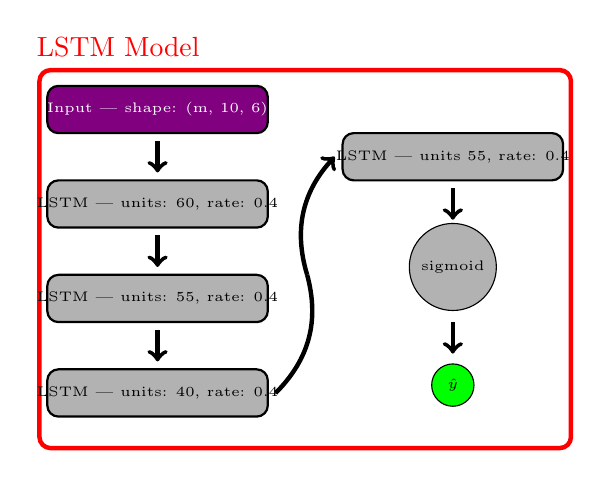
\begin{tikzpicture}
			\node at (1, 4.3) {\textcolor{red}{LSTM Model}};
			\draw [ultra thick, red, rounded corners] (0, -0.8) rectangle (6.75, 4);

			\draw [thick, black, rounded corners, fill=violet] (0.1, 3.8) rectangle
			(2.9, 3.2);
			\node [white] at (1.5, 3.5) {\tiny Input | shape: (m, 10, 6)};

			\draw [ultra thick, ->] (1.5, 3.1) -- (1.5, 2.7);

			\draw [thick, black, rounded corners, fill=black!30] (0.1, 2.6)
			rectangle (2.9, 2.0);
			\node [black] at (1.5, 2.3) {\tiny LSTM | units: 60, rate:
			0.4};

			\draw [ultra thick, ->] (1.5, 1.9) -- (1.5, 1.5);

			\draw [thick, black, rounded corners, fill=black!30] (0.1, 1.4)
			rectangle (2.9, 0.8);
			\node [black] at (1.5, 1.1) {\tiny LSTM | units: 55, rate:
			0.4};

			\draw [ultra thick, ->] (1.5, 0.7) -- (1.5, 0.3);

			\draw [thick, black, rounded corners, fill=black!30] (0.1, 0.2)
			rectangle (2.9, -0.4);
			\node [black] at (1.5, -0.1) {\tiny LSTM | units: 40, rate:
			0.4};

			\draw [ultra thick] (3.0, -0.1) to[bend right] (3.4, 1.4);
			\draw [ultra thick, ->] (3.4, 1.4) to[bend left] (3.75, 2.9);

			\draw [thick, black, rounded corners, fill=black!30] (3.85, 3.2)
			rectangle (6.65, 2.6);
			\node [black] at (5.25, 2.9) {\tiny LSTM | units 55, rate: 0.4};

			\draw [ultra thick, ->] (5.25, 2.5) -- (5.25, 2.1);

			\node [circle, draw, fill=black!30] (c) at (5.25, 1.5) {\tiny sigmoid};

			\draw [ultra thick, ->] (5.25, 0.8) -- (5.25, 0.4);

			\node [circle, draw, fill=green] (c) at (5.25, 0.0) {\tiny $\hat{y}$};
		\end{tikzpicture}
		\end{figure}
\end{frame}

\begin{frame}{Base Model Architectures: GRU}
	\begin{figure}
		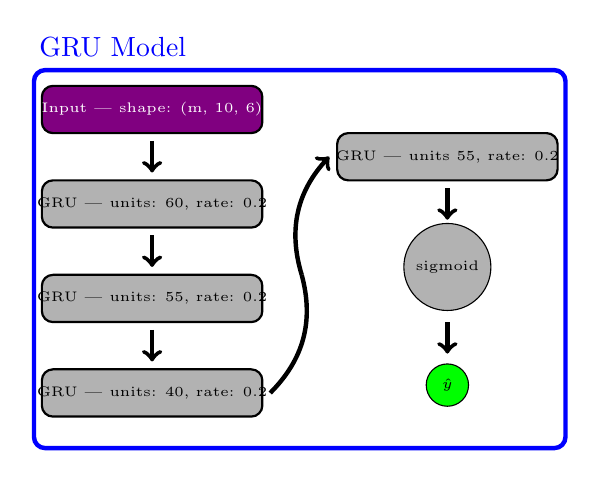
\begin{tikzpicture}
			\node at (1, 4.3) {\textcolor{blue}{GRU Model}};
			\draw [ultra thick, blue, rounded corners] (0, -0.8) rectangle (6.75, 4);

			\draw [thick, black, rounded corners, fill=violet] (0.1, 3.8) rectangle
			(2.9, 3.2);
			\node [white] at (1.5, 3.5) {\tiny Input | shape: (m, 10, 6)};

			\draw [ultra thick, ->] (1.5, 3.1) -- (1.5, 2.7);

			\draw [thick, black, rounded corners, fill=black!30] (0.1, 2.6)
			rectangle (2.9, 2.0);
			\node [black] at (1.5, 2.3) {\tiny GRU | units: 60, rate:
			0.2};

			\draw [ultra thick, ->] (1.5, 1.9) -- (1.5, 1.5);

			\draw [thick, black, rounded corners, fill=black!30] (0.1, 1.4)
			rectangle (2.9, 0.8);
			\node [black] at (1.5, 1.1) {\tiny GRU | units: 55, rate:
			0.2};

			\draw [ultra thick, ->] (1.5, 0.7) -- (1.5, 0.3);

			\draw [thick, black, rounded corners, fill=black!30] (0.1, 0.2)
			rectangle (2.9, -0.4);
			\node [black] at (1.5, -0.1) {\tiny GRU | units: 40, rate:
			0.2};

			\draw [ultra thick] (3.0, -0.1) to[bend right] (3.4, 1.4);
			\draw [ultra thick, ->] (3.4, 1.4) to[bend left] (3.75, 2.9);

			\draw [thick, black, rounded corners, fill=black!30] (3.85, 3.2)
			rectangle (6.65, 2.6);
			\node [black] at (5.25, 2.9) {\tiny GRU | units 55, rate: 0.2};

			\draw [ultra thick, ->] (5.25, 2.5) -- (5.25, 2.1);

			\node [circle, draw, fill=black!30] (c) at (5.25, 1.5) {\tiny sigmoid};

			\draw [ultra thick, ->] (5.25, 0.8) -- (5.25, 0.4);

			\node [circle, draw, fill=green] (c) at (5.25, 0.0) {\tiny $\hat{y}$};
		\end{tikzpicture}
	\end{figure}
\end{frame}

\begin{frame}{Blended Ensemble Architecture}
	\begin{figure}
			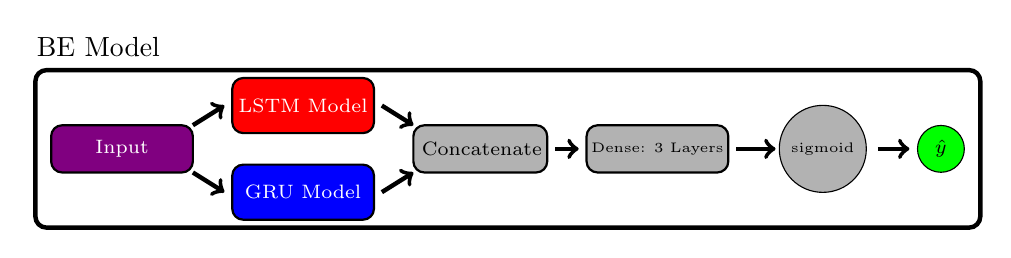
\begin{tikzpicture}
		\node at (0.8, 2.3) {BE Model};
		\draw [ultra thick, black, rounded corners] (0, 0) rectangle (12, 2);

		 \draw [thick, black, rounded corners, fill=violet] (0.2, 0.7)
		 rectangle (2, 1.3);
		 \node [white] at (1.1, 1.0) {\scriptsize Input};

		 \draw [ultra thick, ->] (2, 1.3) -- (2.4, 1.55);
		 \draw [ultra thick, ->] (2, 0.7) -- (2.4, 0.45);

		 \draw [thick, black, rounded corners, fill=red] (2.5, 1.2) rectangle
		 (4.3, 1.9);
		 \node [white] at (3.4, 1.55) {\scriptsize LSTM Model};

		 \draw [ultra thick, ->] (4.4, 1.55) -- (4.8, 1.3);

		 \draw [thick, black, rounded corners, fill=blue] (2.5, 0.8) rectangle
		 (4.3, 0.1);
		 \node [white] at (3.4, 0.45) {\scriptsize GRU Model};

		 \draw [ultra thick, ->] (4.4, 0.45) -- (4.8, 0.7);

		 \draw [thick, black, rounded corners, fill=black!30] (4.8, 0.7)
		 rectangle (6.5, 1.3);
		 \node at (5.67, 1.0) {\scriptsize Concatenate};

		 \draw [ultra thick, ->] (6.6, 1.0) -- (6.9, 1.0);

		 \draw [thick, black, rounded corners, fill=black!30] (7.0, 0.7)
		 rectangle (8.8, 1.3);
		 \node at (7.9, 1.0) {\tiny Dense: 3 Layers};

		 \draw [ultra thick, ->] (8.9, 1.0) -- (9.4, 1.0);

		 \node [circle, draw, fill=black!30] (c) at (10, 1.0) {\tiny
		 sigmoid};

		 \draw [ultra thick, ->] (10.7, 1.0) -- (11.1, 1.0);

		 \node [circle, draw, fill=green] (c) at (11.5, 1.0) {\scriptsize
		 $\hat{y}$};
	\end{tikzpicture}
	\end{figure}

	Blended Ensemble Workflow:
	\begin{enumerate}
		\item Train both the LSTM \& GRU models on the training data
		\item Predict the validation results using each model and concatenate
		\item Train the dense layer on these predictions as input
		\item Predict the test set by running it through the entire procedure
	\end{enumerate}
\end{frame}

\begin{frame}{Resulting Accuracies}
	\begin{table}
	\centering
	\begin{tabular}{c c c c}
		\toprule
		Model & Day 1 Prediction & Day 3 Prediction & Day 5 Prediction\\
		\midrule
		LSTM & 36.25\% & 22.12\% & 17.85\%\\
		GRU & 59.35\% & \textbf{52.67}\% & \textbf{26.75}\%\\
		BE & \textbf{65.12}\% & -- & -- \\
		\bottomrule
	\end{tabular}
\end{table}
	\begin{itemize}
		\item The largest accuracy found was \alert{67\%}
		\item Using fundamental information contributes to this accuracy
	\end{itemize}
\end{frame}

\begin{comment}
\begin{frame}{Simulation Speedup: 100 Runs}
	\begin{columns}
		\column{0.5\textwidth}
		\begin{figure}
			\includegraphics[scale=0.42]{plots/100_run_times.png}
			\caption{Times to simulate 100 models for different optimization
			attempts.}
		\end{figure}
		\column{0.5\textwidth}
		Class definitions:
		\begin{enumerate}
			\item No I/O correction
				\begin{itemize}
					\item (24 cores)
				\end{itemize}
			\item Straight-forward I/O correction
				\begin{itemize}
					\item (24 cores)
				\end{itemize}
			\item Source code \& wizardry
				\begin{itemize}
					\item (24 cores)
				\end{itemize}
			\item Source code \& wizardry
				\begin{itemize}
					\item (36 cores)
				\end{itemize}
		\end{enumerate}
	\end{columns}
\end{frame}

\begin{frame}{Where Did the Speedup Come From?}
	\begin{columns}
		\column{0.5\textwidth}
		\begin{figure}
			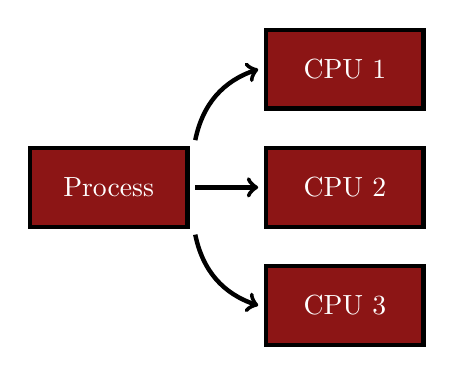
\begin{tikzpicture}
				\draw [ultra thick, fill=cardinalred] (0, 0) rectangle (2, 1);
				\node [white] at (1.0, 0.5) {Process};

                \draw [ultra thick, fill=cardinalred] (3, 1.5) rectangle (5, 2.5);
				\node [white] at (4, 2.0) {CPU 1};
				\draw [ultra thick, ->] (2.1, 1.1) to[bend left] (2.9, 2);

				\draw [ultra thick, fill=cardinalred] (3, 0) rectangle (5, 1);
				\node [white] at (4, 0.5) {CPU 2};
				\draw [ultra thick, ->] (2.1, 0.5) -- (2.9, 0.5);

				\draw [ultra thick, fill=cardinalred] (3, -0.5) rectangle (5, -1.5);
				\node [white] at (4, -1) {CPU 3};
				\draw [ultra thick, ->] (2.1, -0.1) to[bend right] (2.9, -1.0);
			\end{tikzpicture}
			\caption{Multiprocessing involves sending portions of a process off
			to separate CPUs.}
		\end{figure}
		\column{0.5\textwidth}
		\begin{itemize}
			\item Original fix:
				\begin{itemize}
					\item Cease load and save of saturation, pressure, \& model
						text files for each iteration
					\item Small files, so speed up was limited
				\end{itemize}
			\item Advanced fix:
				\begin{itemize}
					\item \textit{TensorFlow} requires weights to be loaded as
						h5 files
					\item \alert{Very} large files loaded on each model run
					\item Changed \textit{TensorFlow} source code to fix this
					\item An assortment of other optimizations
				\end{itemize}
		\end{itemize}
	\end{columns}
\end{frame}

\begin{frame}{Simulation Speedup: ES-MDA}
	\begin{columns}
		\column{0.5\textwidth}
		\begin{figure}
			\includegraphics[scale=0.42]{plots/ESMDA_times.png}
			\caption{Times to simulate ES-MDA with 10 assimilation steps.}
		\end{figure}
		\column{0.5\textwidth}
		Class definitions:
		\begin{enumerate}
			\item Original version with I/O
				\begin{itemize}
					\item (24 cores)
				\end{itemize}
			\item Optimized version: no I/O
				\begin{itemize}
					\item (24 cores)
				\end{itemize}
			\item Optimized version: no I/O
				\begin{itemize}
					\item (36 cores)
				\end{itemize}
		\end{enumerate}

		Notes:
		\begin{itemize}
			\item 24-36 cores has a small difference due to overhead
			\item Can increase up to 108 cores
			\item Equivalent to 1100 runs
		\end{itemize}
	\end{columns}
\end{frame}

\begin{frame}{Is This Ensemble Collapse?}
	\begin{figure}
		\centering
		\includegraphics[scale=0.46]{plots/errors_2_2_new.png}
		\caption{Uncertainty reduction for a sensor system of two wells and two
		locations per well. The question is: is it too good to be true?}
	\end{figure}
\end{frame}

\begin{frame}[t]{Histograms at Each Layer}
	\begin{columns}
		\column{0.5\textwidth}
		\begin{figure}
			\begin{tikzpicture}
				\node at (0, 0)
				{\includegraphics[scale=0.40]{plots/base_model.png}};

				\begin{onlyenv}<1>
					\draw [ultra thick, red] (-2.40, 1) rectangle (2.20, 1.20);
				\end{onlyenv}

				\begin{onlyenv}<2>
					\draw [ultra thick, red] (-2.40, 1) rectangle (2.20, 0.35);
				\end{onlyenv}

				\begin{onlyenv}<3>
					\draw [ultra thick, red] (-2.40, 0.35) rectangle (2.20, -0.05);
				\end{onlyenv}

				\begin{onlyenv}<4>
					\draw [ultra thick, red] (-2.40, -0.05) rectangle (2.20, -0.50);
				\end{onlyenv}

				\begin{onlyenv}<5>
					\draw [ultra thick, red] (-2.40, -0.50) rectangle (2.20, -0.88);
				\end{onlyenv}
			\end{tikzpicture}
		\end{figure}

		\column{0.5\textwidth}
		\begin{onlyenv}<1>
		    \begin{figure}
		    	\includegraphics[scale=0.42]{plots/hists_layer0.png}
		    \end{figure}
		\end{onlyenv}

		\begin{onlyenv}<2>
			\begin{figure}
				\includegraphics[scale=0.42]{plots/hists_layer1.png}
			\end{figure}
		\end{onlyenv}

		\begin{onlyenv}<3>
			\begin{figure}
				\includegraphics[scale=0.42]{plots/hists_layer2.png}
			\end{figure}
		\end{onlyenv}

		\begin{onlyenv}<4>
			\begin{figure}
				\includegraphics[scale=0.42]{plots/hists_layer3.png}
			\end{figure}
		\end{onlyenv}

		\begin{onlyenv}<5>
			\begin{figure}
				\includegraphics[scale=0.42]{plots/hists_layer4.png}
			\end{figure}
		\end{onlyenv}
	\end{columns}
\end{frame}

\begin{frame}{Variogram Access}
	\begin{columns}
		\column{0.5\textwidth}
		\begin{figure}
			\includegraphics[scale=0.10]{plots/simple_stats.png}
			\caption{Recently provided to me when requesting variogram
			information.}
		\end{figure}
		\column{0.5\textwidth}
		Provided to me:
		\begin{itemize}
			\item $\phi$ and k values from Lively Grove well
			\item Access to well log information
		\end{itemize}

		Making new models:
		\begin{itemize}
			\item Was told to get variograms 'soon'
			\item Quickly making ad-hoc ensembles: 10,000 models
			\item Trying to use well logs to get corr. lengths
		\end{itemize}
	\end{columns}
\end{frame}

\begin{frame}{Notes from Last ISC Meeting}
	\begin{itemize}
		\setlength\itemsep{1em}
		\item Mansor RokRok \& James Domico are to get me some variograms
		\item Roland assured me we would get an ensemble
			\begin{itemize}
				\item Or the means to make it, i.e., statistics
			\end{itemize}
		\item Steven is worried modelers may be over-fitting by $\phi/k$
			relations
		\item \alert{One Earth}: they now know where to put one monitoring well
			\begin{itemize}
				\item Concerned with locating an optimal place for the
					injector here
				\item Asked if we could also do this
			\end{itemize}
	\end{itemize}
\end{frame}
\end{comment}
\end{document}
